\documentclass[]{article}
\usepackage{lmodern}
\usepackage{amssymb,amsmath}
\usepackage{ifxetex,ifluatex}
\usepackage{fixltx2e} % provides \textsubscript
\ifnum 0\ifxetex 1\fi\ifluatex 1\fi=0 % if pdftex
  \usepackage[T1]{fontenc}
  \usepackage[utf8]{inputenc}
\else % if luatex or xelatex
  \ifxetex
    \usepackage{mathspec}
  \else
    \usepackage{fontspec}
  \fi
  \defaultfontfeatures{Ligatures=TeX,Scale=MatchLowercase}
\fi
% use upquote if available, for straight quotes in verbatim environments
\IfFileExists{upquote.sty}{\usepackage{upquote}}{}
% use microtype if available
\IfFileExists{microtype.sty}{%
\usepackage[]{microtype}
\UseMicrotypeSet[protrusion]{basicmath} % disable protrusion for tt fonts
}{}
\PassOptionsToPackage{hyphens}{url} % url is loaded by hyperref
\usepackage[unicode=true]{hyperref}
\PassOptionsToPackage{usenames,dvipsnames}{color} % color is loaded by hyperref
\hypersetup{
            pdftitle={Package Stereo3D},
            pdfauthor={Vinod Kumar Singh, Yang Liu and Deyou Zheng},
            colorlinks=true,
            linkcolor=blue,
            citecolor=Blue,
            urlcolor=Blue,
            breaklinks=true}
\urlstyle{same}  % don't use monospace font for urls
\usepackage[margin=1in]{geometry}
\usepackage{color}
\usepackage{fancyvrb}
\newcommand{\VerbBar}{|}
\newcommand{\VERB}{\Verb[commandchars=\\\{\}]}
\DefineVerbatimEnvironment{Highlighting}{Verbatim}{commandchars=\\\{\}}
% Add ',fontsize=\small' for more characters per line
\usepackage{framed}
\definecolor{shadecolor}{RGB}{248,248,248}
\newenvironment{Shaded}{\begin{snugshade}}{\end{snugshade}}
\newcommand{\KeywordTok}[1]{\textcolor[rgb]{0.13,0.29,0.53}{\textbf{#1}}}
\newcommand{\DataTypeTok}[1]{\textcolor[rgb]{0.13,0.29,0.53}{#1}}
\newcommand{\DecValTok}[1]{\textcolor[rgb]{0.00,0.00,0.81}{#1}}
\newcommand{\BaseNTok}[1]{\textcolor[rgb]{0.00,0.00,0.81}{#1}}
\newcommand{\FloatTok}[1]{\textcolor[rgb]{0.00,0.00,0.81}{#1}}
\newcommand{\ConstantTok}[1]{\textcolor[rgb]{0.00,0.00,0.00}{#1}}
\newcommand{\CharTok}[1]{\textcolor[rgb]{0.31,0.60,0.02}{#1}}
\newcommand{\SpecialCharTok}[1]{\textcolor[rgb]{0.00,0.00,0.00}{#1}}
\newcommand{\StringTok}[1]{\textcolor[rgb]{0.31,0.60,0.02}{#1}}
\newcommand{\VerbatimStringTok}[1]{\textcolor[rgb]{0.31,0.60,0.02}{#1}}
\newcommand{\SpecialStringTok}[1]{\textcolor[rgb]{0.31,0.60,0.02}{#1}}
\newcommand{\ImportTok}[1]{#1}
\newcommand{\CommentTok}[1]{\textcolor[rgb]{0.56,0.35,0.01}{\textit{#1}}}
\newcommand{\DocumentationTok}[1]{\textcolor[rgb]{0.56,0.35,0.01}{\textbf{\textit{#1}}}}
\newcommand{\AnnotationTok}[1]{\textcolor[rgb]{0.56,0.35,0.01}{\textbf{\textit{#1}}}}
\newcommand{\CommentVarTok}[1]{\textcolor[rgb]{0.56,0.35,0.01}{\textbf{\textit{#1}}}}
\newcommand{\OtherTok}[1]{\textcolor[rgb]{0.56,0.35,0.01}{#1}}
\newcommand{\FunctionTok}[1]{\textcolor[rgb]{0.00,0.00,0.00}{#1}}
\newcommand{\VariableTok}[1]{\textcolor[rgb]{0.00,0.00,0.00}{#1}}
\newcommand{\ControlFlowTok}[1]{\textcolor[rgb]{0.13,0.29,0.53}{\textbf{#1}}}
\newcommand{\OperatorTok}[1]{\textcolor[rgb]{0.81,0.36,0.00}{\textbf{#1}}}
\newcommand{\BuiltInTok}[1]{#1}
\newcommand{\ExtensionTok}[1]{#1}
\newcommand{\PreprocessorTok}[1]{\textcolor[rgb]{0.56,0.35,0.01}{\textit{#1}}}
\newcommand{\AttributeTok}[1]{\textcolor[rgb]{0.77,0.63,0.00}{#1}}
\newcommand{\RegionMarkerTok}[1]{#1}
\newcommand{\InformationTok}[1]{\textcolor[rgb]{0.56,0.35,0.01}{\textbf{\textit{#1}}}}
\newcommand{\WarningTok}[1]{\textcolor[rgb]{0.56,0.35,0.01}{\textbf{\textit{#1}}}}
\newcommand{\AlertTok}[1]{\textcolor[rgb]{0.94,0.16,0.16}{#1}}
\newcommand{\ErrorTok}[1]{\textcolor[rgb]{0.64,0.00,0.00}{\textbf{#1}}}
\newcommand{\NormalTok}[1]{#1}
\usepackage{graphicx,grffile}
\makeatletter
\def\maxwidth{\ifdim\Gin@nat@width>\linewidth\linewidth\else\Gin@nat@width\fi}
\def\maxheight{\ifdim\Gin@nat@height>\textheight\textheight\else\Gin@nat@height\fi}
\makeatother
% Scale images if necessary, so that they will not overflow the page
% margins by default, and it is still possible to overwrite the defaults
% using explicit options in \includegraphics[width, height, ...]{}
\setkeys{Gin}{width=\maxwidth,height=\maxheight,keepaspectratio}
\IfFileExists{parskip.sty}{%
\usepackage{parskip}
}{% else
\setlength{\parindent}{0pt}
\setlength{\parskip}{6pt plus 2pt minus 1pt}
}
\setlength{\emergencystretch}{3em}  % prevent overfull lines
\providecommand{\tightlist}{%
  \setlength{\itemsep}{0pt}\setlength{\parskip}{0pt}}
\setcounter{secnumdepth}{0}
% Redefines (sub)paragraphs to behave more like sections
\ifx\paragraph\undefined\else
\let\oldparagraph\paragraph
\renewcommand{\paragraph}[1]{\oldparagraph{#1}\mbox{}}
\fi
\ifx\subparagraph\undefined\else
\let\oldsubparagraph\subparagraph
\renewcommand{\subparagraph}[1]{\oldsubparagraph{#1}\mbox{}}
\fi

% set default figure placement to htbp
\makeatletter
\def\fps@figure{htbp}
\makeatother

\usepackage{setspace}\singlespacing
\usepackage{float}

\title{Package `Stereo3D'}
\author{Vinod Kumar Singh, Yang Liu and Deyou Zheng}
\date{2020-02-28}

\begin{document}
\maketitle
\renewcommand{\abstract}{}
\begin{abstract}
.\\
\textbf{Title}: Stereo3D\\
\textbf{Type}: Package\\
\textbf{Version}: 1.0.0

\textbf{Description}: Using stereo images to enrich 3D visualization.\\
\textbf{Author}: Vinod Kumar Singh, Yang Liu and Deyou Zheng\\
\textbf{Maintainer}: The package maintainer
\href{mailto:vinodsinghjnu@gmail.com}{\nolinkurl{vinodsinghjnu@gmail.com}}\\
\textbf{License}: MIT + file LICENSE~\\
\textbf{Encoding}: UTF-8\\
\textbf{LazyData}: true\\
\textbf{Depends}: R (\textgreater{}= 3.6.2), plyr, plotrix, tools, rgl,
scatterplot3d.\\
\textbf{RoxygenNote}: 7.0.2\\
\textbf{Suggests}:devtools, knitr, rmarkdown.\\
\textbf{VignetteBuilder}: knitr.\\
\textbf{URL}: \url{https://github.com/bioinfoDZ/Stereo3D}\\
\textbf{BugReports}: \url{https://github.com/bioinfoDZ/Stereo3D/issues}
\end{abstract}

\newpage

\tableofcontents

\subsection{1. Introduction:}\label{introduction}

Visualization in three-dimensional (3D) space is a standard and critical
process for examining the complex structure of high dimensional data.
Stereo imaging technology can be adopted to enhance 3D representation of
any complex data, especially those consisting mostly of points and
lines. We illustrate the simple steps that are involved and strongly
encourage others to implement it in their own visualization software. To
facilitate its application, we have also created a new software that can
convert a regular 3D scatterplot or network figure to a stereo image

\subsection{2. Concept:}\label{concept}

When 2D-image of original data and the slightly rotated data are viewed
side by side a 3D illusion is created due to two perspectives of the
same object.

The original set of coordinates \((X, Y, Z)\) can be rotated
(counter-clockwise direction) by an angle \(\theta\) along Y-axis using
the rotation matrix \(R_y (\theta)\). The new set of coordinates is
obtained as

\[
\begin{aligned}
\begin{bmatrix}
X^` \\ Y^` \\ Z^` \\ 1
\end{bmatrix}  & =
R_y (\theta) \cdot
\begin{bmatrix}
X \\ Y \\ Z \\ 1
\end{bmatrix}  \\
& =
\begin{pmatrix}
cos \theta & 0 & -sin \theta & 0\\
0 & 1 & 0 & 0\\
sin \theta & 0 & cos \theta & 0\\
0 & 0 & 0 & 1
\end{pmatrix} \cdot
\begin{bmatrix}
X \\ Y \\ Z \\ 1
\end{bmatrix}
\end{aligned}
\]

\subsection{3. Availability and
Installation}\label{availability-and-installation}

The development version of \texttt{Stereo3D} package is available at
\url{https://github.com/bioinfoDZ/Stereo3D} and can be installed as

\begin{Shaded}
\begin{Highlighting}[]
\CommentTok{# install.packages("devtools")}
\NormalTok{devtools}\OperatorTok{::}\KeywordTok{install_github}\NormalTok{(}\StringTok{"bioinfoDZ/Stereo3D"}\NormalTok{,}\DataTypeTok{build_vignettes =} \OtherTok{FALSE}\NormalTok{ )}
\end{Highlighting}
\end{Shaded}

\subsection{4. Functions}\label{functions}

\subsubsection{4.1 Stereo3D}\label{stereo3d}

\paragraph{\texorpdfstring{\textbf{Description}}{Description}}\label{description}

Create Stereoscopic 3D image of the given data.

\paragraph{\texorpdfstring{\textbf{Usage}}{Usage}}\label{usage}

\texttt{Stereo3D(data\_file=sample\_data\_file,\ stereo\_angle,\ distance,\ connection\_file)}

\paragraph{\texorpdfstring{\textbf{Arguments
}}{Arguments }}\label{arguments}

\begin{itemize}
\tightlist
\item
  \texttt{data\_file}: A tab seperated file with \texttt{".tsv"}
  extension and having five columns (\texttt{index}, \texttt{X},
  \texttt{Y}, \texttt{Z} and \texttt{Color}) of the data. Where,
  \texttt{X}, \texttt{Y} and \texttt{Z} represent cordinates of a
  datapoint, \texttt{Color} is the label of the given data point and
  \texttt{index} clolumn have the index information of the datapoints.
\item
  \texttt{stereo\_angle}: angle by which 3D data to be rotated along
  Y-axis. \texttt{Default:\ 5\ degree}
\item
  \texttt{distance}: Distance or gap between the two stereo images.
\item
  \texttt{connection\_file}: A tab seperated file (optional). Where,
  \texttt{first} and \texttt{second} column has indices of start and end
  points (from \texttt{data\_file}) of a connection respectively.
\end{itemize}

\paragraph{\texorpdfstring{\textbf{Details}}{Details}}\label{details}

The dataset is rotatated by a given angle along the Y-axis and a
Stereoscopic 3D scatter plot image is creaated.

\paragraph{\texorpdfstring{\textbf{Value}}{Value}}\label{value}

\begin{itemize}
\tightlist
\item
  Create Stereoscopic 3D plot with
  \texttt{input\ data\ filename\ prefix} and \texttt{\_Stereo.pdf}
  extention.
\item
  Interactive 3D plot of the above image, which can be zoomed and rotated by draging the mouse.
\end{itemize}

\paragraph{\texorpdfstring{\textbf{Examples}}{Examples}}\label{examples}

\begin{verbatim}
> connection_fileName=system.file("extdata", "connection_file.tsv",
package = "Stereo3D", mustWork = TRUE)
> sample_data_file=system.file("extdata", "sample_3D_data.tsv",
package = "Stereo3D", mustWork = TRUE)

> Stereo3D(data_file=sample_data_file, stereo_angle=5, distance=0,
connection_file=connection_fileName) # dataset stereo image is created
and saved in "sample_3D_data_Stereo.pdf"
\end{verbatim}

\paragraph{Output}\label{output}

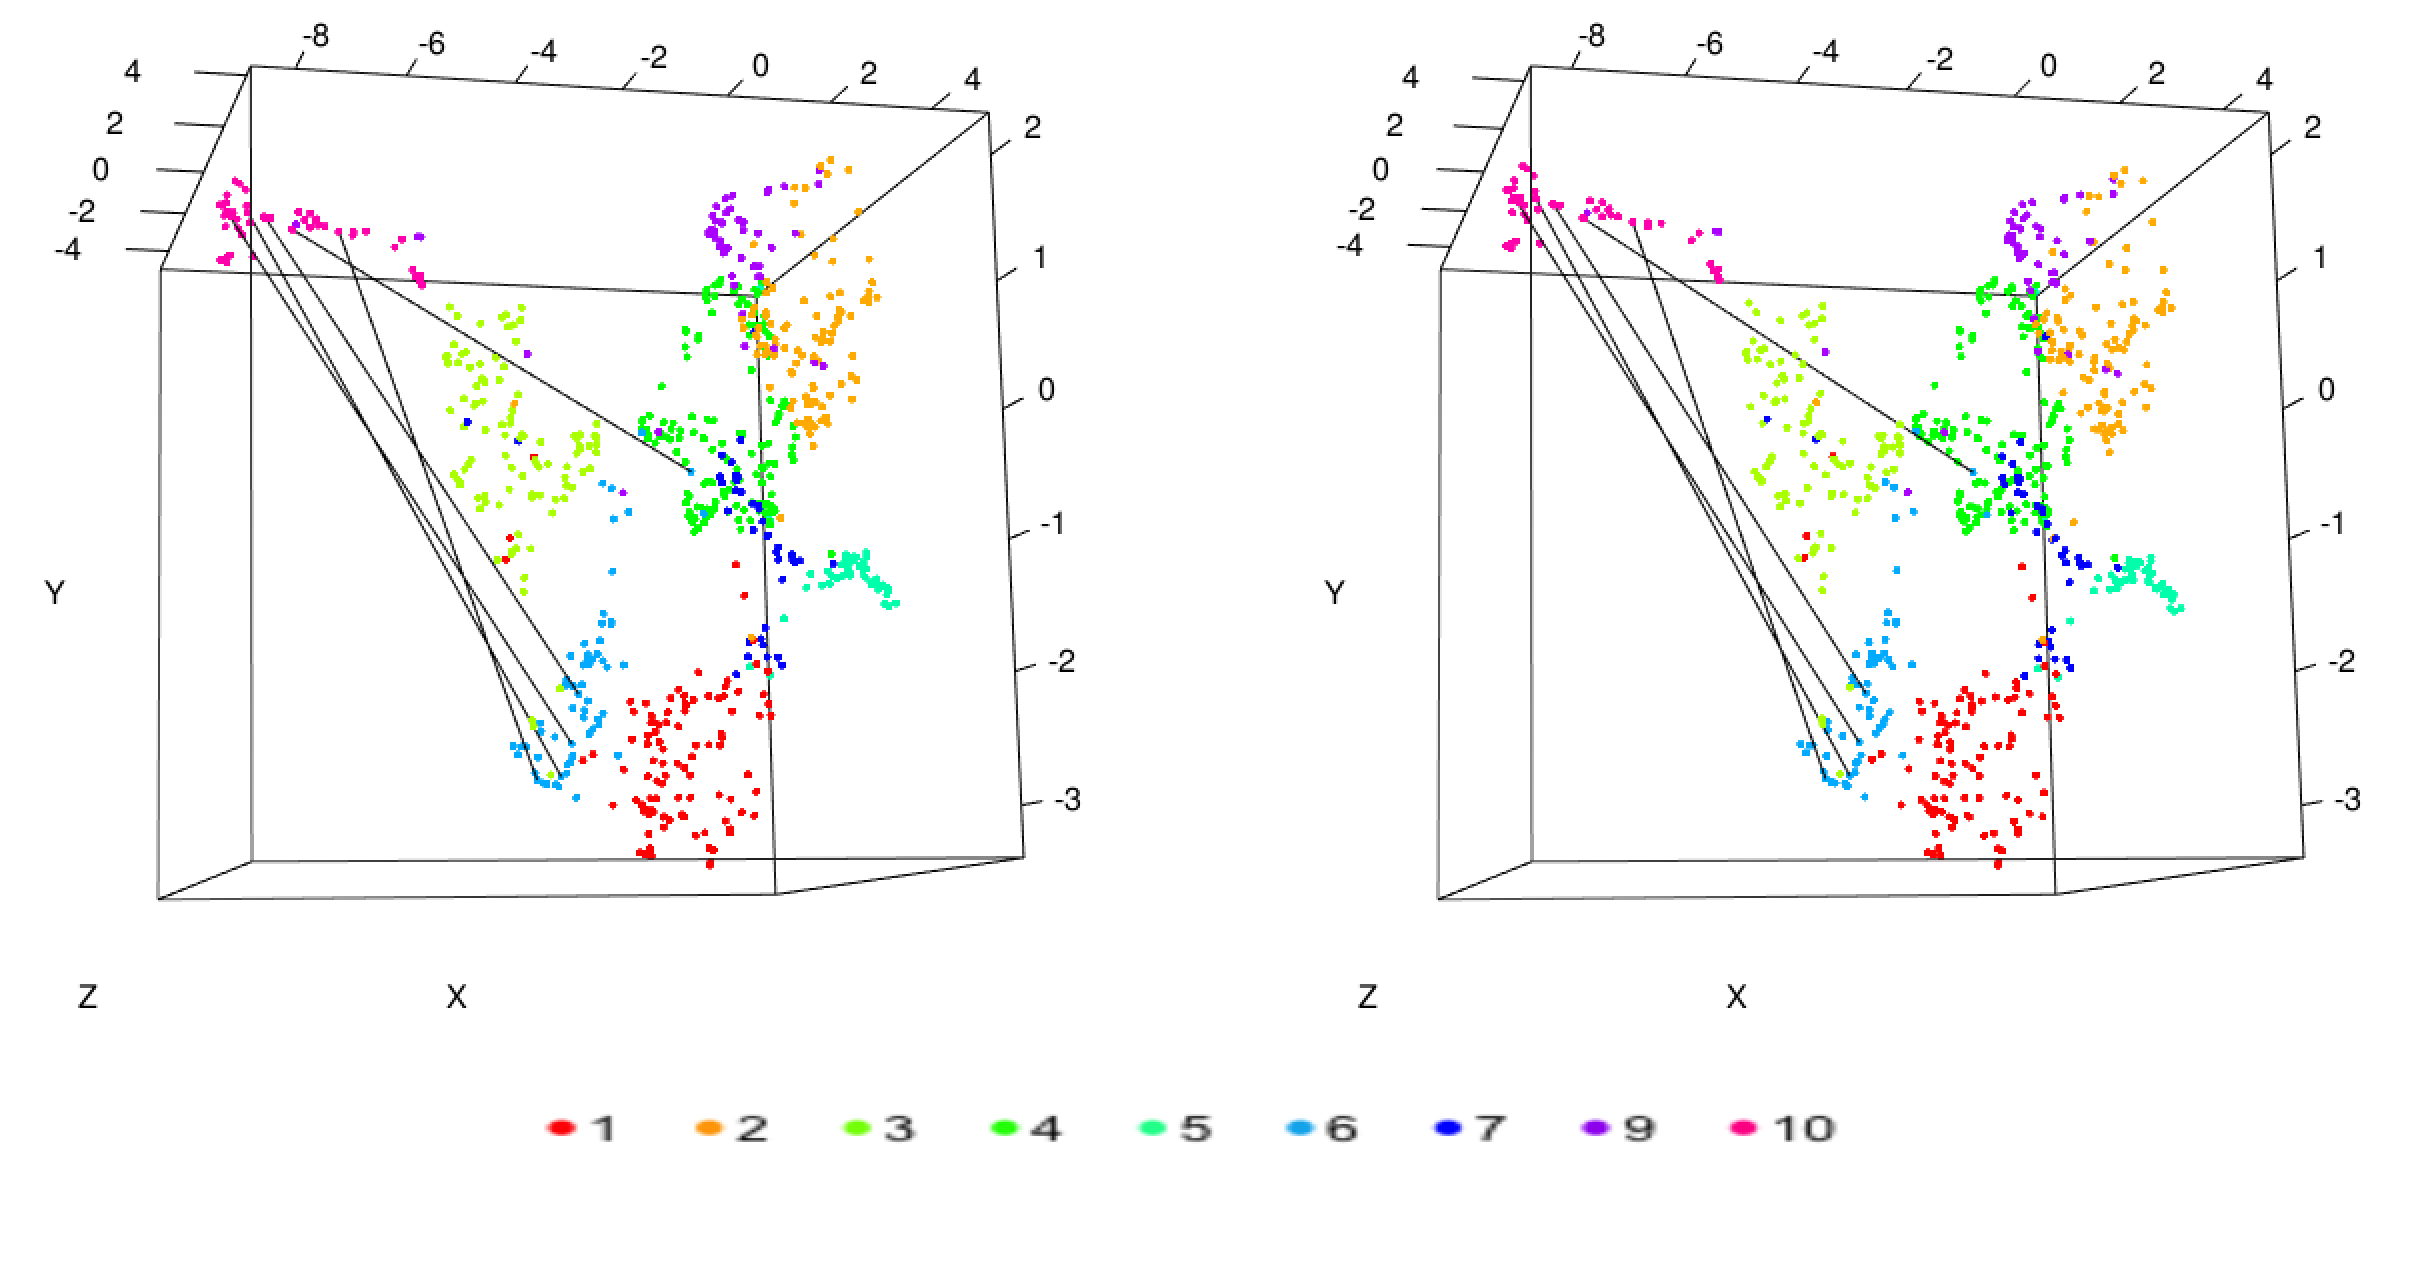
\includegraphics{../sample.png} 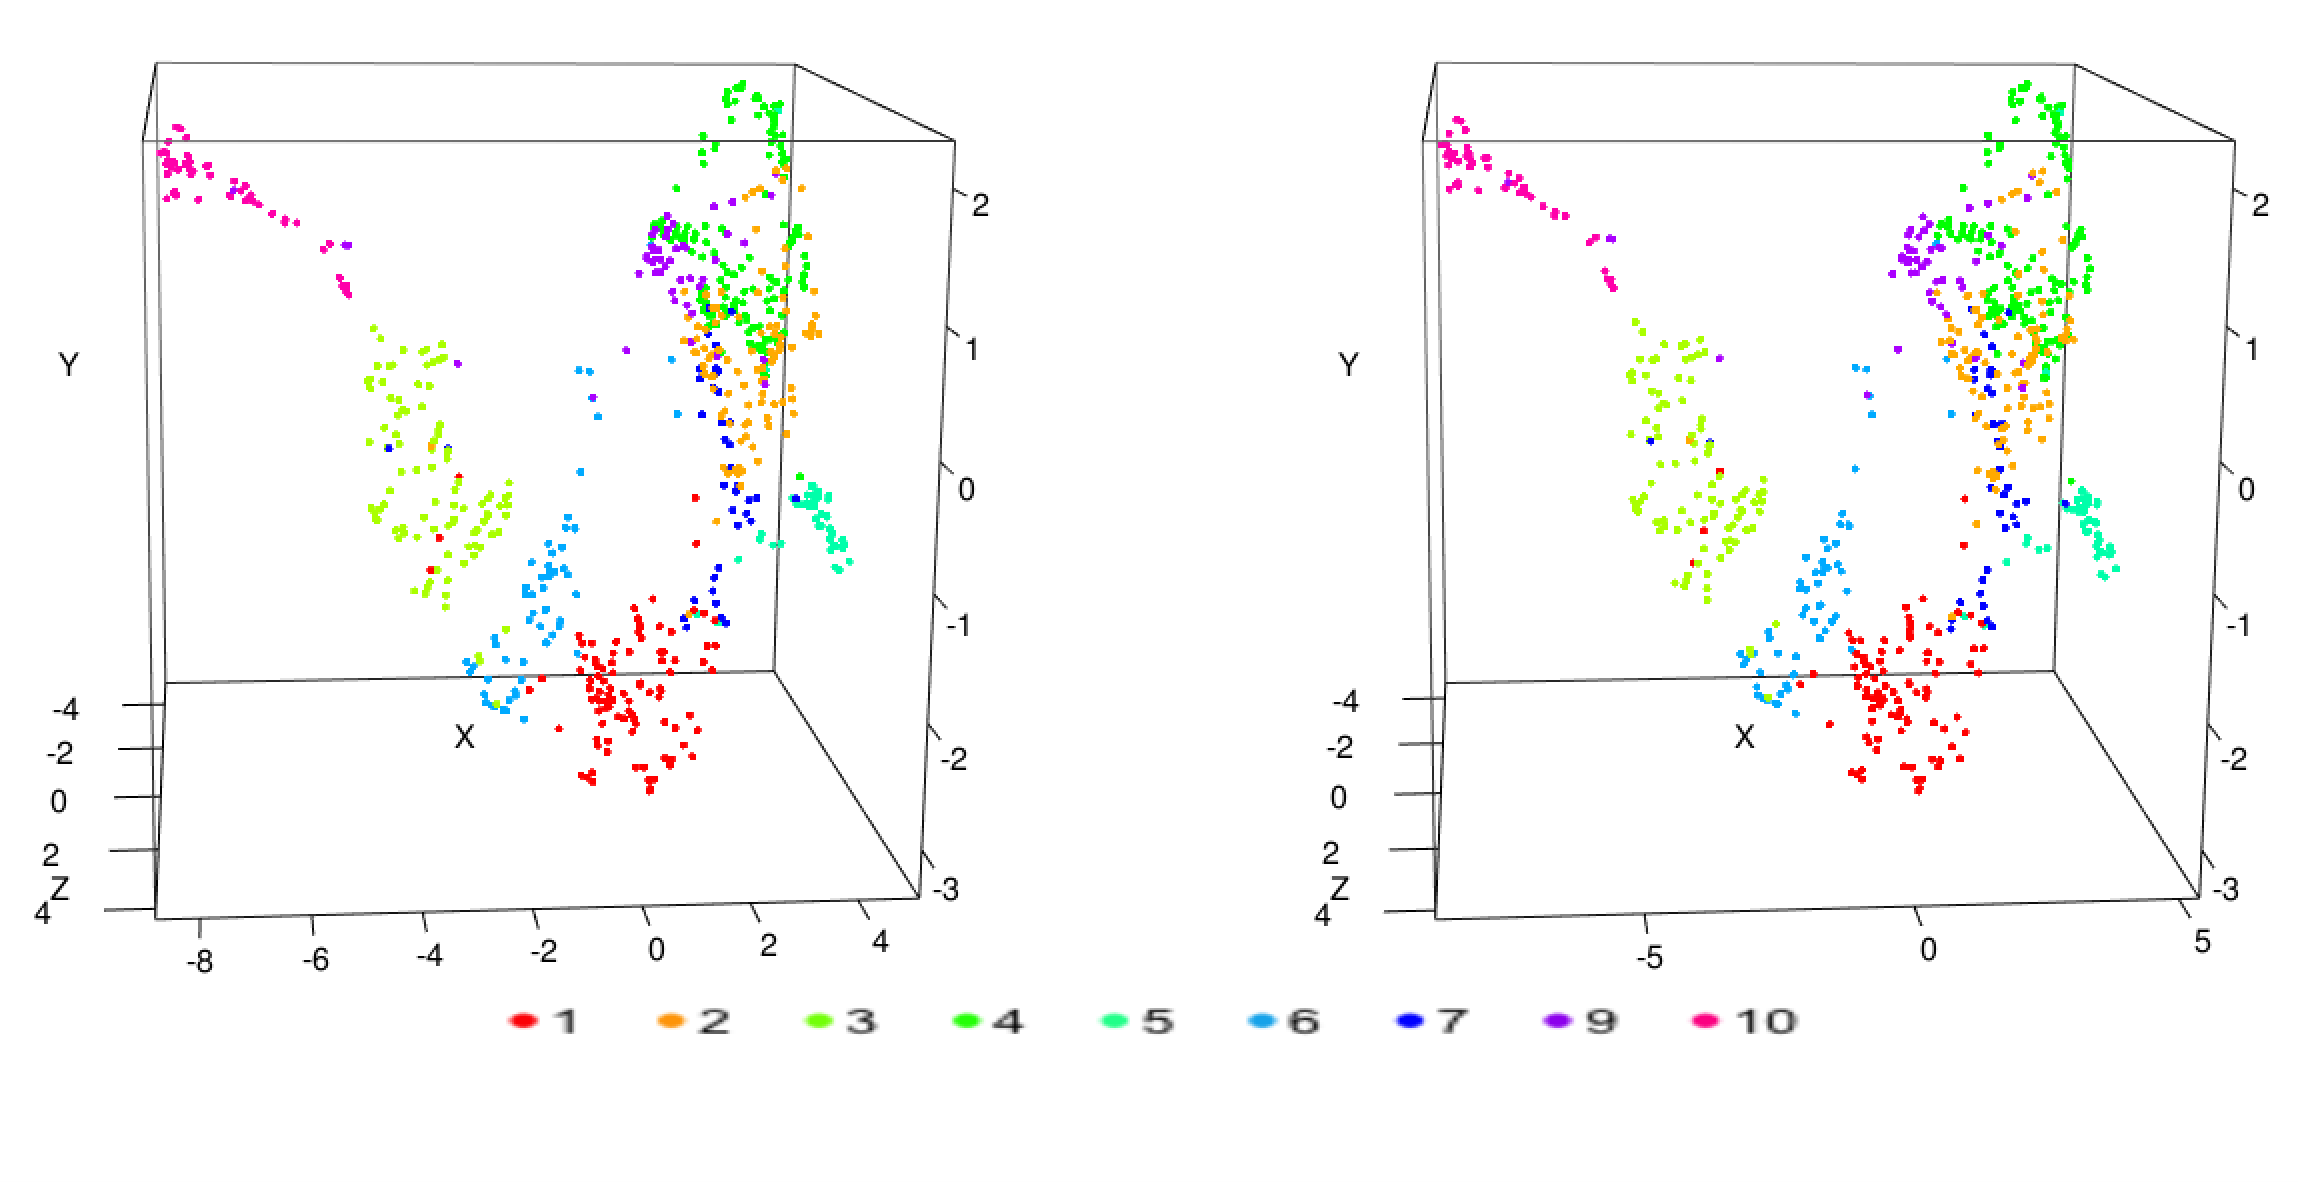
\includegraphics{../sample_scatter.png}

\begin{figure}
\centering
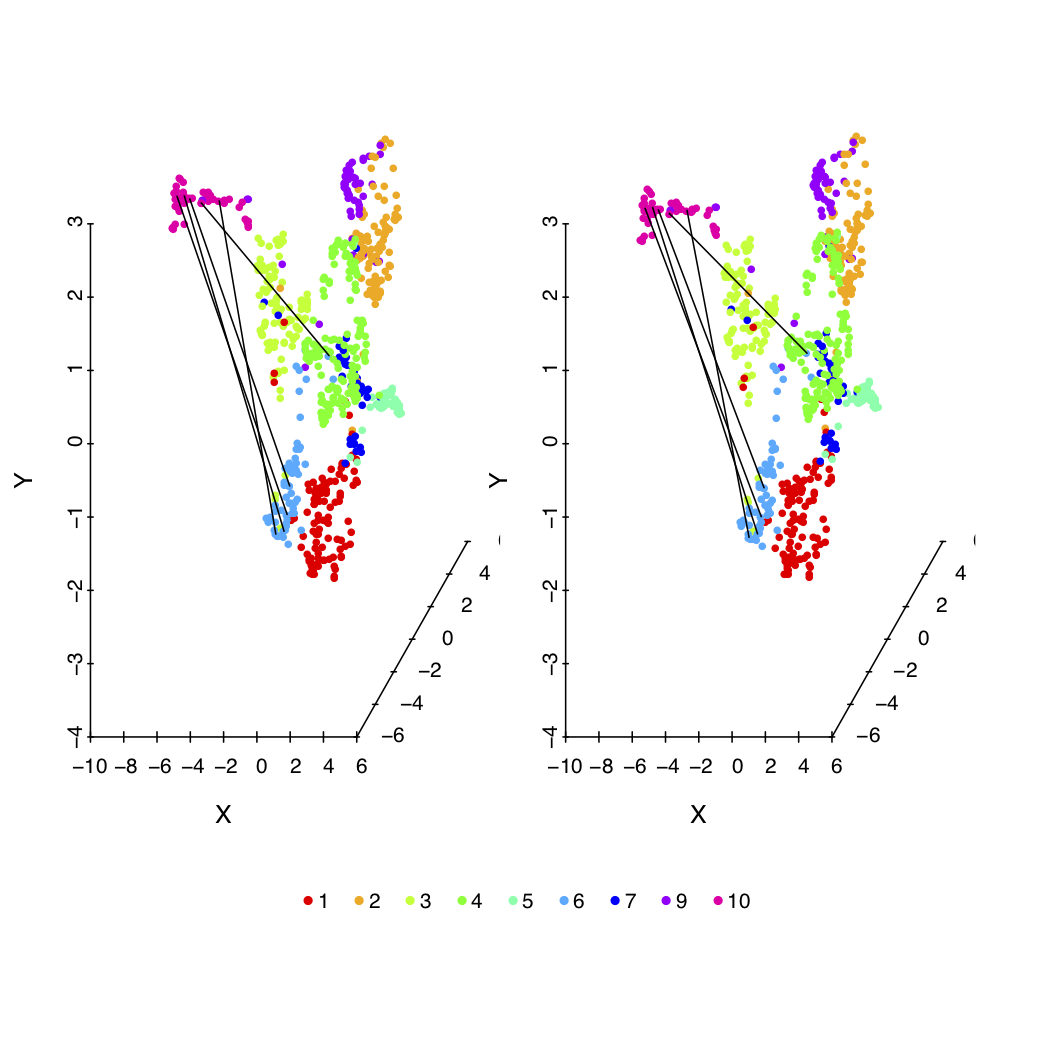
\includegraphics{../sample_3D_data_Stereo_net.png}
\caption{``Output: Sterio Image 2''}
\end{figure}

\end{document}
